\begin{figure}[!h]
\centering
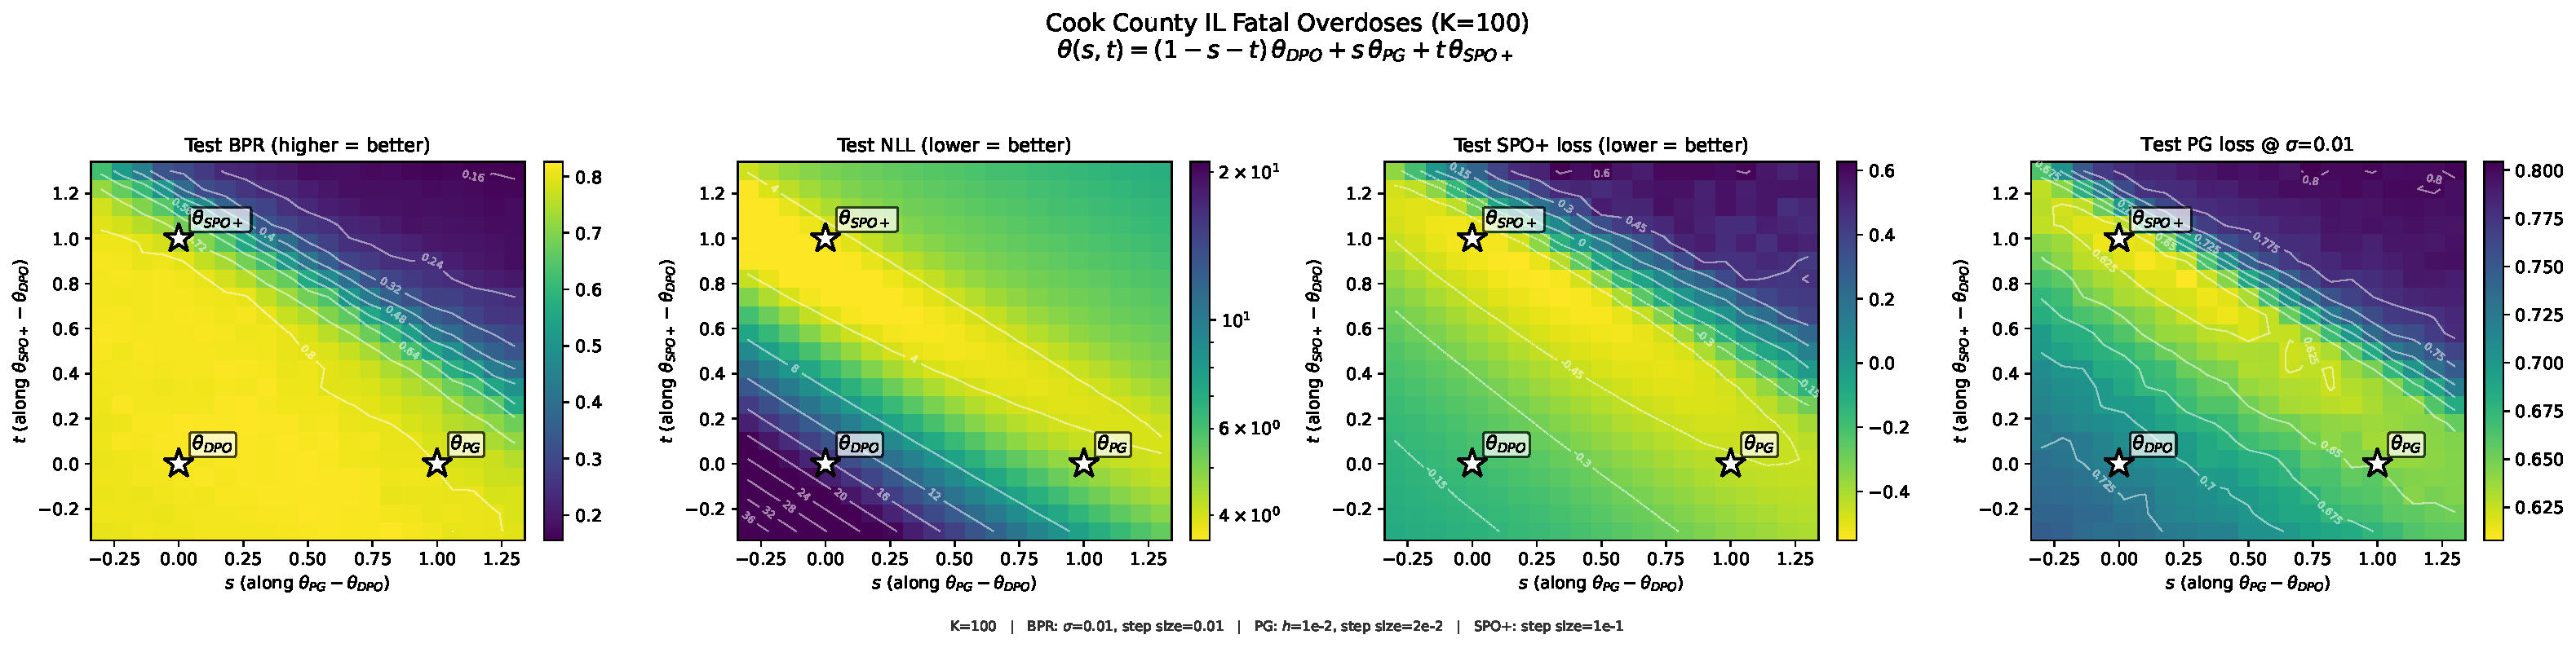
\includegraphics[width=\linewidth]{figures/hyperplane_landscape_cook.pdf}

% Tighten space before caption (local to this figure)
\vspace{-0.3em}
\setlength{\abovecaptionskip}{2pt}
\setlength{\belowcaptionskip}{0pt}
\caption[Top-K site selection: loss landscape on the affine hyperplane spanning $\theta_{DPO}$, $\theta_{PG}$, and $\theta_{SPO+}$.]{
\textbf{Top-K site selection on Cook County, IL ($K{=}100$).}
Heldout-test metrics on the affine hyperplane $\theta(s,t)=(1{-}s{-}t)\theta_{DPO}+s\,\theta_{PG}+t\,\theta_{SPO+}$. From left: BPR (higher better); SPO+ surrogate on per-instance decision loss $\langle z, \bm{y}_t\rangle$; SPO+ surrogate on per-instance BPR objective $\langle z, \bm{y}_t\rangle/C_t$; PG surrogate on $\langle z, \bm{y}_t\rangle$; PG surrogate on $\langle z, \bm{y}_t\rangle/C_t$. Lower is better for the surrogate panels. $s, t$ extended beyond $[0,1]$ to expose the surrounding landscape; stars mark the three trained solutions. The BPR task setup is given in App.~\ref{app:bpr_setup}.
}%endcaption
\label{fig:topK_interpolation_main}
\end{figure}

In Section~\ref{sec:synth} we considered two complementary questions about decision-aware methods: which solutions a method's loss landscape prefers, and which solutions the method is capable of reaching by gradient descent. We turn the same lens on the real-world top-K tasks of Chapter~\ref{chap:daml}~\citep{heuton2025decisionaware}, where direct minimization of BPR via a perturbed-optimizer estimator (which we call ``DPO'' in this section) was reported to outperform two alternative surrogate methods, PG and SPO+.

Are PG and SPO+ unable to reach as low a BPR as DPO because of their landscape (they prefer a $\theta$ with worse BPR), because of their optimization (they get stuck in a local minimum), or because they were applied to a different objective (they reach the right $\theta$ for the wrong loss)?

The distinction between BPR and the surrogates' default objective is normalization. BPR is the per-instance ratio
\begin{align}
\text{BPR}(z, \bm{y}_t) = \frac{\langle z, \bm{y}_t\rangle}{C_t},
\quad C_t = \sum_{s \in \textsc{TopKIDs}(\bm{y}_t, K)} y_{s,t},
\end{align}
where $C_t$ is the oracle's reach at time $t$. Off-the-shelf PG and SPO+ surrogates are derived for the unnormalized $\langle z, \bm{y}\rangle$ and have no built-in division by $C_t$. Per-instance the two objectives have identical argmin in $\theta$, but at the dataset level $C_t$ varies considerably across timesteps and tracts, so the two averaged objectives reweight instances differently and prefer different $\theta$.

Fig.~\ref{fig:topK_interpolation_main} resolves which explanation applies on the Cook County opioid task. Applied to the unnormalized per-instance decision loss (panels 2 and 4), both SPO+ and PG produce landscapes whose argmin sits away from $\theta_{DPO}$. Applied to the BPR-normalized per-instance objective (panels 3 and 5), the same surrogates produce landscapes that closely resemble the BPR landscape (panel 1), with their argmin near $\theta_{DPO}$. The same pattern holds for Massachusetts and the aerial-survey wildlife task in App.~\ref{app:topK} (Fig.~\ref{fig:topK_interpolation_6panel}).

PG and SPO+ are capable of reaching the same kind of solution as direct BPR optimization on these tasks, provided they are given the BPR-normalized per-instance objective. What appeared in Chapter~\ref{chap:daml} as a method-intrinsic advantage of DPO is, on these tasks, training-objective alignment with the evaluation metric. The practical recommendation is to derive the surrogate's training signal from the normalized per-instance objective when the evaluation metric is normalized.
